\documentclass{standalone}

\usepackage[compat=1.1.0]{tikz-feynman}

\begin{document}

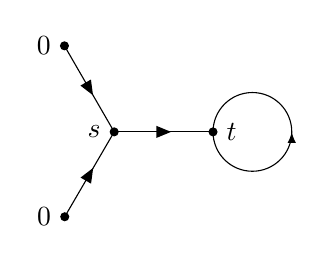
\begin{tikzpicture}
    \begin{feynman}
        \diagram [small, horizontal=a to b] {
            a[dot,label=left:$s$] --[fermion] b[dot,label=right:$t$],
            x[dot,label=left:$0$] --[fermion] a,
            y[dot,label=left:$0$] --[fermion] a,
        };
    \end{feynman}

    \draw[
        decoration={markings, mark=at position 0 with {\arrow{latex}}},
        postaction={decorate}
    ]
    (b) ++ (0.5,0) circle (0.5);
\end{tikzpicture}

\end{document}